\documentclass[12pt, Arial]{article}   	
\title{Teaching a Class to Grade Itself using Game Theory}
\author{Nick Kaashoek and William Wu}
\date{\today}
\usepackage[margin=1in]{geometry}
\usepackage{parskip}
\usepackage{graphicx}
\setlength{\parindent}{15pt}
\begin{document}
\maketitle
\section{Introduction}
Over the past few years, there has been a tremendous increase in the popularity of MOOCs (Massive Open Online Courses), as well the importance of MOOCs to education as a whole. Popular MOOC systems such as Coursera or EdX are well funded, which explains their rapid growth: 60 million dollars were invested in EdX when it started~\cite{canmoocsreducecc}. However, the MOOC's main importance comes from its scalability. MOOCs are able to educate massive numbers of students from anywhere in the world~\cite{makingsenseofmoocs}: By the end of 2012, 1.7 million students had attended a course through Coursera~\cite{swotanalysisofmoocs}. The sheer number of students leads to high student-professor ratios that can reach 150,000:1 in some courses.

High student-professor ratios lead to problems for professors. Professors are simply unable to grade hundreds of thousands of submissions. Currently, two types of solutions are used to remedy the problem: automated grading and peer grading. Automated grading relies on machines to grade assignments. However, machines can only check certain types of answers (i.e. multiple choice), severely limiting the depth of the questions asked~\cite{rightandwrongmoocs}. Even though automated grading for written essays is an active area of research with much recent progress, a usable solution does not yet exist~\cite{automatedsystemssuck}. On the other hand, peer grading can grade any type of question, but a system utilizing it could easily be ``hacked'' by the students~\cite{makingsenseofmoocs}. Although both of these systems are interesting concepts, they are limiting or inaccurate in practice~\cite{howaccurateispeergrading}.

The problem of grading large numbers of submissions is important to solve. Without a solid solution, MOOCs cannot provide efficient feedback for their students, rendering them unable to effectively evaluate their knowledge. Because this limits their learning abilities, it is imperative to create an efficient system that enables students to receive feedback to learn efficiently.

There have been many attempts at solving such an important problem~\cite{autograding}~\cite{edxsoftware}. However, this work introduces what previous attempts lack: a rigorous mathematical analysis of the system using tools from game theory and mechanism design. This work sets a concrete set of constraints that a grading system must satisfy to mitigate student incentive to cheat, as well as a concrete benchmark to analyze the efficiency of various systems. Together, these create a concrete measure for evaluating peer grading systems in terms of efficiency (how much time the professor and students spend grading) and fairness for the students (how accurate their final scores are). Having this measurement model is a large contribution in itself, because it allows comparison between different systems. Although a theoretical model cannot predict exactly what will happen in practice, game theory and mechanism design have a history of generally determining mechanisms that work in practice from ones that do not. Mechanisms that do not follow game theoretic constraints may work in the short-term, but they will be exploited if possible in the long term~\cite{boycottfinal}.
%[Note from Matt and Christos: 1) mention that coming up with a model is itself a big contribution, because now we can compare the quality of two different mechanisms. 2) Mention that certainly theory is not a perfect predictor of what will happen in practice, but that game theory and mechanism design (and all the assumptions used in this work) have a history of ``calling good mechanisms good and bad mechanisms bad''. Also, solutions that do not satisfy game theoretic constraints may work for a while, but in the long run if a system can be exploited, eventually it will be. See here for an interesting example of this: http://www.insidehighered.com/news/2013/02/12/students-boycott-final-challenge-professors-grading-policy-and-get]

Game theory allows the creation of a unified system of assumptions that simulate student behavior in a class. The grading system can be viewed as a ``game'' where the set of ``rules'' are known to everyone and the ``players'' --- the students --- ``play'' the game in order to get the best possible result. Using the assumptions and rules, game theory can predict how students will behave when they ``play''. This way, mechanism efficiency and effectiveness cam be proved, allowing the evaluation of different sets of rules.

The difficulty of the problem lies in finding an incentive for students to spend time to grade assignments of others who they don't care about. Incentivizing students seems simple at first: let the professor give bonus points to students who grade, for example. However, this may not return anything useful because a clever student will just take the points and assign a generic grade (i.e. they will just give every assignment a 100). The next step would be to implement simple checking: e.g. have each paper be graded by two students who both receive bonus points if their grades match. This case may work if the students are isolated, but clever students will still just give all papers 100. This way, their papers will match those of other clever students, giving them points without grading. These examples show that properly incentivizing graders can be a difficult task. The main purpose of this work is to devise mechanisms which avoid these problems, allowing for work to be distributed efficiently.

As demonstrated by the above examples, the difficulty of the problem lies in the complex behavior of selfish human beings. Because human nature dictates that people will do whatever is in their best interest and may try to outsmart the system, coming up with a strict set of rules to encourage the desired behavior can be quite challenging. A mechanism should be made as simple as possible, but the above examples show that a small amount of simplicity must be sacrificed to obtain a system that can't be manipulated.

This research opportunity is made interesting by the complexity of human nature as well as its necessity for practical use. This paper will cover the thought process of mechanisms leading up to the final mechanism of grading, as well as explain the final mechanism and its implications. All mechanisms and related calculations will be presented. Section 2 describes the mathematical definition of the problem as well as its rules and assumptions.

\section{Materials and Methods}
\subsection{The Scenario}
In our trying to find a solution to the professor's problem, we created a scenario in which our solution applies to a single assignment. This means that our system will have to be repeated for every assignment, instead of performing on a global scale. In such a "round" of grading, there are $n$ students, who each bring one ungraded paper to the professor. These ungraded papers are like the input for a function. Each of these papers has an objective score $o_i\mid 0<o_i<100$. This is the score the professor would give out. Our mechanism then grades the paper, and outputs these grades. After one "round" each student receives a grade $g_i$ and after performing $w_i$ units of work, where for one paper, $w_i=1$. The professor is index 0.
\subsection{Assumptions}
To create the models that are used to predict the behavior of the students, a set process was used each time. To begin with, a set of assumptions is created. These assumptions are used to explain how students will act in a given situation; for example, one assumption could be that students want good grades. This is a logical assumption that is likely true, as all the assumptions are, and can be used to classify the behavior of the students in a model. The same set of assumptions can be used for multiple models, which will allow us to evaluate different models side by side. To begin with, a simple set of assumptions was created:
\begin{enumerate}
	\item Students want good grades
 	\item Doing work makes students unhappy
  	\item Students want to be happy
 	\item Students only care about their final happiness
  	\item The happiness of a student is only affected by their grade and the amount of work they do
\end{enumerate}
However, we wanted to create a mathematical solution, so these assumptions need to be changed into math terms. The result of this is as follows:
\begin{enumerate}
  \item Students all share a common happiness function, $H(g)$, where \emph{g} represents the grade the students received, and the output is their happiness. w.l.o.g. $H(0)=0$
  \item Students can grade others' work perfectly but doing so costs one unit of happiness. Therefore after grading $W$ papers, a student's happiness can be expressed as $H(g)-W$
  \item Students want to maximize their final happiness, expressed as $H(g)-W$
  \item Students only care about the expectation of their final happiness, which, put in game theory terms, makes them risk neutral (i.e, if $H(x)=10$ and $H(y)=5$, then getting x and y each with 50 percent chance, gives a happiness of 7.5).
  \item The final happiness depends only on the grade assigned to the student and the amount of effort exercised. It doesn't depend on the score of others
\end{enumerate}

\subsection{Why?}
There are two questions that need to be addressed, first, why is happiness important, and second, why are the scores of others not important? The importance of happiness lies in the fact that it provides a way to compare different outcomes; effectively allowing us to show definitively which of two models is better. The reasoning for not caring about friends is due to the relatively low impact they have on someone's grades and happiness, as well as the incredible complexity the model would have to account for with this considered.
\subsection{First major objective}
No student can deviate from the truthful strategy to improve his happiness. In math terms, if by acting honestly student i grades $w_i$ papers and gets a grade of $g_i$ there shouldn't be any way for the student to spend $w'_i$ units of effort and get a score $g'_i$ where $H(g'_i)-w'_i > H(g_i)-w_i$.

\subsection{Benchmark}
%Efficiency objective%
The next step is to create a system that will allow multiple different models to be compared and evaluated side by side; in other words, a benchmark needs to be created. To do this, two things need to be addressed: how accurate the grades the mechanism produces are, and how happy people are. Because happiness can be directly expressed as a function of work, the two things that need to be evaluated are how accurate the grades are, and how much work is being done. As such, the benchmark becomes a sum of the amount of work done by the person doing the most work and the maximum deviation from the correct grades; the lower the sum, the more efficient the mechanism. In mathematical terms we want to minimize the function $max_{i \ge 1} |H(g_i)-H(o_i)| + max_{i \ge 0} w_i$ in the worst possible case.

Caring about the workload is just as important as caring about accurate grades. If the system was purely based on minimizing only the work done by a single person, everyone could just get 100. Likewise, if the system was purely based on maximizing grade accuracy, the professor could grade everything. In order to properly model the problem to achieve a solution that is reasonable, both aspects of the problem need to be considered.

% We now have a well defined problem that we need to solve. Of course the set of assumptions might not be very realistic as we will so we 

Once a simple set of assumptions and a benchmark were created, the assumptions need to be further developed into a true model that will become the ``''rules'' of the game. To do this, a model was created that will simulate the environment of a classroom, based on the observations of students inside real classes. This turned the list of assumptions from the 
simple into:
%Repeat above corrections%
\begin{enumerate}
\item When grading, $w_i=0 \oplus w_i=1$
\item For all students, $g_i \neq o_i$
\item Students all share a common happiness function, $H(g)$, where \emph{g} represents the grade the students received, and the output is their happiness. w.l.o.g. $H(0)=0$
\item Students can grade others' work perfectly but doing so costs one unit of happiness. Therefore after grading $W$ papers, a student's happiness can be expressed as $H(g)-W$
\item Final happiness is unaffected by other people, only affected by $g_i$ and $w_i$
\item Doing work costs one unit of happiness, so after grading a paper, a student's happiness can be expressed as $H(g)-W$,W is number of work units used
\item Students only care about the expectation of their final happiness, which, put in game theory terms, makes them risk neutral.
\item For a given student in $N$, that student has contact with all other students in $N$.
\end{enumerate}
Put simply:
\begin{enumerate}
\item Students cannot "half bake" an assignment
\item Students can't always get the exact objective score
\item Students want good grades
\item Students don't like grading
\item Students are selfish
\item Doing work costs 1 unit of effort
\item Students are risk neutral with respect to happiness
\item All students can talk to each other
\end{enumerate}

These assumptions provide the necessary environment to begin creating a mechanism, as they state everything that is necessary to understand how students behave. Simply put, every assignment has a grade from 1-100, and whatever the professor says goes. Every student has a different capacity for grading, and as such not everyone will be able to correctly grade very assignment, but they can only choose to either grade or not grade. All students are capable of communicating with each other, and will do so, and the rest is from the simple set of assumptions.

Because it would be illogical to start creating a mechanism to encompass all of these assumptions, every mechanism grows in complexity, with the first one being the most simple. Throughout the design process, the assumptions were changed to allow for simplicity, which allows for the creation of simpler models. The complex set of assumptions were always kept in mind, however.

\section{Discussion}
With this research, the goal was to create a mechanism that fulfilled our two goals; incentivizing students to play the "game" the way they were meant to, and to efficiently and effectively grade the assignments of these students. Although our mechanisms are not truly realistic, the significance of them cannot be denied. The mechanisms created by the end of the research came very close to realism, with only one factor missing, and could still be implemented in a classroom environment where all students are capable of grading others assignments efficiently.

The work done in creating these mechanisms further builds upon that which has been done before to try and answer the same question of grading large numbers of papers. Much of the previous work done to address this problem involves creating automated mechanisms that simple spit out machine-assigned grades. These solutions, as stated previously, are inefficient and often produce unsatisfactory results. By creating these mechanisms using game theory, it has been shown that computers do not need to be relied upon to grade papers, opening the way for others to create game theory driven solutions to this problem.

Also, by taking the happiness of the students into account, it can be almost guaranteed that these mechanisms are better for the students than automated grading, or any other solutions attempted before. Many of the complaints that students give out include something along the lines of the fact that they cannot give feedback on their feedback, a problem in the Coursera system~\cite{theproblemswithpeergradingincoursera}. This problem is fixed in our mechanism by allowing the students to appeal their grades and to have multiple rounds of grading. Other commonly expressed problems such as the variability of feedback are also addressed by these mechanisms, which prevent this from happening by having a rigid set of justifications required. This means that students cannot simply pass on a paper with the word "good," they must rather take the time to explain why they took off any points they did, or why they gave the paper a perfect score.

Besides making the students happier than they are in other peer grading systems, the mechanisms that result from this research also provide more accurate and legitimate grades for the students. In current peer grading schemes, it is easy for students to just "game" the system and fake their way through a course. Giving anonymous feedback, for example, does not encourage students to be honest, rather, it gives them a reason to be \emph{dis}honest~\cite{theproblemswithpeergradingincoursera}. This allows students to dishonestly grade the work of others, as well as just give whomever they want a better grade than that person actually deserves. In our mechanisms, however, these problems are solved by removing anonymity and adding incentives to make students behave honestly, no matter who they are grading.

Aside from fixing many problems that students have with other peer grading systems, our mechanisms also address the unhappiness and inconsistency caused by the grading given out by machines. One key problem that machines have is that they always look at the same thing in a paper, meaning that they can be easily "gamed" and fooled into thinking something is better than it acutely is~\cite{robogradingproblems}. Not only does this make the system inconsistent, but any student who is lacking something that is in the list of requirements the machine checks for can be unfairly given a poor grade, making them unhappy. By solving both of these problems with the mechanisms that were created, it has been demonstrated the peer grading, at least for the moment, is all in all better for education that automated grading.

Not only do the mechanisms developed in this research improve upon the efficiency of automated grading systems, but they also help to remove the dominance that automated grading has placed on grading large courses. By providing a system that fixes many of the problems with current automated grading systems, these mechanisms help to show that automated grading is not the only way to solve the problem of grading online courses. Because automated grading, at the moment, is not as efficient and robust as it needs to be to prevent students from creating unfair situations, this is something that is necessary to show because automated grading is simply not good enough with today's technology.

By creating a mechanism that is, in theory, more efficient than both current peer grading systems and automated grading systems, it has been shown that there is still room for improvement in the grading of online courses. By showing this, a renewed interest in the field can be created, which could lead to others developing more mechanisms that will improve the general education of students in these courses. As the ultimate goal of this research is to accomplish this, the idea that the mechanisms not only accomplish this, but also open the road for others to do so is a marked success.

All in all, with the final mechanism, all of the goals that were set up were accomplished, with only total realism absent from the design. With this final mechanism, it has been shown that it is possible to create a mathematically driven and effective design that can solve a problem that needs to be solved. Not only is this something that has not been done before, but it opens the way for others to build upon this work, something that could eventually lead to the creation of a perfect solution. 

However important the creation of these mechanisms is, arguably more important to the future development of further solutions is the creation of a realistic and robust model. Without a model, many of the mechanisms mentioned would have been impossible to create, and would certainly not work as well as they do. The creation of a model is essential in game theory as it provides the outline for how the "players" of a given game will act under any set of circumstances. As such, by creating a good model, this research has undergone the trouble of providing a way for anyone to predict how students will behave. 

Not only did this research lead to the creation of a good model, but it also led to the creation of a benchmark. The creation of a benchmark is important because it allows two or mechanisms to be compared side by side, and it allows theorists to definitively determine which of these mechanisms is superior. With this, it becomes possible to compare the results of this research to the results of others, and also allows future work to be done by others. Not only does a benchmark allow the research done here to be compared to that of others, but it allows two totally independent mechanisms not derived from this research to be compared, which could lead to a universal system of evaluating peer grading systems.

Both of these are major contributions towards further developments in the field of research this problem takes place in, primarily game theory. By doing so, grading mechanisms across online courses will constantly be able to evolve and improve with contributions from anyone. By creating the benchmark and model, all mechanisms will undergo a uniform set of evaluations that will allow online course systems to determine which system is the best out of any proposals. By doing so, this research has opened up a road for many game theorists to develop and analyze new ideas that will lead to improvements in student happiness and results from online courses.

Due to the numerous possibilities the creation of a model and benchmark can lead to for future research, it is clear that they are the most important results gained from this research. Without them, nothing else could have been done, and no future mechanisms could be created that would be able to be analyzed in the same way that these were. Due to the importance of future research in this field, it was imperative that this research led to more solutions in the future, so that the problem that was identified would be quickly and efficiently solved.

Although the models presented by this research are not completely realistic, they do show that there is much room for improvement in the area of grading online courses, and that it is possible to take a strictly mathematical approach at designing a mechanism, and then implementing it using computer science. By showing that this is possible, a huge amount of potential for future research has been opened, primarily due to the creation of a benchmark and model. With these tools, other game theorists can create their own mechanisms, and compare them to those of others around the world.

Aside from improving previous research done in this field, this research also supports the idea that many others have proposed: that peer grading is more efficient than automated grading. When EdX first introduced its automated grading system, many were skeptical of the idea, and had right to be. For this reason, systems such as coursera have yet to adopt this, and instead default to peer grading. As many people suspected, and as this research confirms, peer grading can indeed be more efficient than automated grading when implemented correctly, simply because the A.I. of current machines cannot handle the many different ways a student can answer an open ended question.

Human judgement has always been superior to that of a machine, and this research continues to support that idea. As powerful as automated grading can be in practice, when it comes to theory, peer grading is simply more efficient. This means that with the right mechanism, such as the ones proposed by this research, so, in practice peer grading should be superior to automated grading. All in all, this research has opened doors for game theorists to make improvements to current grading schemes, and also provides mechanisms that are a distinct improvement over current peer and automated grading systems.
\section{Results}
%[Note from Matt and Christos: Add some discussion about the benchmark: why do you care about workload? Why do you care about accurate grades? If you just care about workload, give everyone 100. If you just care about grades, have the professor grade everything. Need to consider both to properly model the problem.]
Once the rules and assumptions have been defined and the benchmark determined, different grading mechanisms can be created and tested. This is where mechanism design and game theory comes into play. Mechanism design is used to create a system that satisfies a set of constraints and achieves a certain purpose. Then, game theory is used to mathematically predict student behavior to benchmark such a system. Starting from the simplest and most obvious approaches, various mechanisms were created, tested, and refined upon in an iterative process that spanned several months. The end result is fairly complete, although there are still questions to be answered in future work.

\section{The Calibration Mechanism}

This mechanism is quite unrealistic, but not by such a degree that it is unimaginable. Because of this, it was possible to create a perfect solution if the problem took place in this situation.

\subsection{Mechanism}
In the mechanism, the professor grades one paper, called \emph{X}. The professor then distributes all the student's papers randomly among the students, while making sure that no student receives his or her own paper. Every student is also given a copy of \emph{X}.


The professor then tells the students that ``Out of the two papers you were given, one of them has been graded by me, and the other hasn't. If you fail to give the correct grade for the one I graded, then you will receive a 0.'' The students then go about their business grading the papers, and individually report the grades they gave out to the professor. Then, just like the professor promised, if the students graded the pre-graded, or \emph{calibrated} paper incorrectly, then that grader gets a 0 on the assignment. If they graded correctly, their assigned grade is guaranteed to be at least some minimum value.

\subsection{Why it Works}
G is the maximum of \{ some minimum value, the assigned grade \}.

The happiness of one student grading one paper is equivalent to $$\frac{H(G)+H(0)}{2}-1$$ Because the students have a 0.5 chance of getting a 0, and a one-half chance of getting G.

If they grade both papers, their happiness will be equal to $$H(G)-2$$Because they spent two units of energy, and are guaranteed to get G.

If they grade neither then the happiness will be $$H(0)$$ Because they automatically get a 0, but spend no energy.

This means that if $H(G) - 2 > H(0)$, then student will grade both papers. So, for the professor to guarantee that the students use effort and obtain the correct grades, he or she would choose a minimum value such that $H(G) > H(0) + 2$.
\subsection{Results}
The teacher expends one unit of effort, and the students each spend 2, as long as the teacher set the minimum value high enough.
Everything above $H^{-1}(2)$ will be graded correctly, while everything below it will receive a score of $H^{-1}(2)$.
This means that the maximum deviation is $H^{-1}(2)$, because this is the score that might be given to someone who deserves a 0. Expressed in happiness units, the value is 2.
The means that the value of the objective function in this case is 4, a very low value, which shows how effective this solution is.

\subsection{Problems}
The goal for this mechanism was to make it more realistic while still making it simple to understand, and have a simply solution that would be easy for students to understand. There is now a mechanism that works very well in an unrealistic scenario, so we moved on to a new mechanism. 

\section{Improved Calibration Mechanism}
The major change made in this mechanism was one to assumption number 11. Now assumption 11 reads as follows:
\emph{All students are able to communicate with each other}

This provides a very different scenario than the original mechanism, because now students will be able to figure out which papers are calibrated. However, it would be better to try and generalize the previous solution and apply it to the new mechanism, which leads to the following scheme.

\subsection{Mechanism}
The first attempt to apply a solution to this mechanism was a near carbon copy of the previous scheme.
The class is arranged in a virtual circle, where every student grades the papers of the \emph{k} students to the right of them. The professor also grades every \emph{kth} paper starting from some random point in the circle. If a student mis-grades the calibrated paper, they get a 0, otherwise they get the maximum of their objective score and the minimum value from the previous mechanism.

\subsection{Why it Works}
In this scheme, because of the overlapping papers, the students have no better way of figuring out which papers are calibrated than random guessing, even though they can all communicate with each other. As such, there are 3 options for the students.

1) They can grade 0 papers, giving them a happiness of $H(0) = 0$

2) They can grade all the papers they are assigned, giving them a happiness of $H(g) - k$

3) They can grade i papers giving them a happiness of $(k-i)\div k \cdot H(G)-i$. This means that it is always worse to grade i, because happiness from grading i is equal to i times happiness for grading 0 plus i-k times happiness for grading k.

\subsection{Results}
Even though the students can communicate with one another, they will have no way to determine which paper is calibrated, and are thus best off grading all the papers.

\subsection{Problems}
The major problem with this method is the amount of work. The professor has to grade $\frac{n}{k}$ papers, which can be massive in a class of 1000+ students. For this reason a different mechanism was necessary.

\section{The Deduction Mechanism}
In the new mechanism, a different strategy was created; one that would ideally work better than the previous ones.

\subsection{Mechanism}
For each assignment, a new assignment is created to evaluate the performance of the graders. Every student receives 2 papers from different people, so that each paper overlaps with one other person, and every paper is distributed twice. The student then chooses how many points to subtract, and writes a justification for each one of these points. Graders are then given a contribution score from 1 to -1. From each of the 2 assignments they grade, they get their points deducted / total points deducted-0.5. Then, if the original writers of the papers can appeal their grade if they are unhappy with it. The professor will grade the paper, and if any of the graders were wrong, they get a 0. To compute the final score, the grader's final grade on the assignment is calculated as follows: 4 points times their contribution score are added or subtracted to H(the student's assigned grade). (Then the student's grade is converted from Happiness to an actual score).

\subsection{Why it Works}
The grader's have two choices, they can either grade the papers, or not grade them.

If the grader does not grade the paper, what score should he give it?

If they take off any points, the points will surely be refuted by the professor during the regrade.
So if they take off any points, they will get a 0 on the grading assignment.
If the grader's give it 100, they might get 50 if the other grader also gives it 100. If he gives it anything else, the original grader will get 0.
$$$$
If the grader does grade the paper, what score should he give it?

If he gives it a lower score, they throw away free points, and if they give it a lower score there is a risk of them getting a 0 because the scores could be refuted. So, giving it the correct score is the best because it guarantees at least a 50.

So assuming that the student's partner gives the paper a 100, which is the best thing they could do if they don't grade, then
	If they don't grade the paper, they don't use any effort. So the student's happiness will H(the student's grade on the original assignment). Contribution score = 0
	If they do grade, they use 1 unit of effort by default. But, the student's happiness will be H(the student's grade on the original assignment) + 3. Contribution score = 1
	
If the grader's partner gives the paper its true grade:
	If the grader doesn't grade the assignment, they will give it a 100 and so the grader's contribution score is -1. So their happiness is H(their original grade) - 4.
	If the grader does grade the assignment, they and their partner gave the same grades, so they get a contribution score of 0. This means that their happiness is H(their original grade). 
	
Therefore, it is in everyone's best interest to honestly grade the paper.

\subsection{Results}
Assuming that everyone acts in the dominant strategy behavior, the maximum work for teacher is 0, the maximum work done for students is 2. 
Because everyone honestly grades the papers, the maximum deviation is 0.
So, the objective function is 2, which is even better than the first mechanism.

\subsection{Problems}
Although the result that was produced for the previous mechanism is rather good, it encourages very harsh competition between students, and would make the classroom environment feel very negative. This means that finding a different solution to the same problem was necessary, in which students are placed in positive competition, instead of the negative one formed by trying to find the most mistakes

\section{The Flag Mechanism}
For the next mechanism, all of the assumptions were kept the same, and simply tried to find a way to better the feeling of negative competition.
\subsection{Mechanism}
Start by having each paper get graded by two people. Then, the original writer of this paper chooses which of the two grades he / she would like to have, and looks over the justifications for losing any points on both papers. If they see that any of these justifications are incorrect, they flag the paper and send it to the professor. Following this, the paper they chose to have is sent to a third party, who grades the paper, and checks if their grade is close to the one that was given to the paper. If it isn't, the paper is sent to the professor. After everything that needs to be flagged has been, the professor grades all the flagged papers, and rewards people who were correct with a 2 point bonus. If no papers from any group were flagged, every grader in that group gets two points. Final grades are whatever the person chose if there was no flagging, or whatever the professor gave them if there was.
\subsection{Why it Works}
To find out how efficient this mechanism is, two things needed to be analyzed:
1) Is everyone an honest flagger?
$$$$
2) Do the graders grade honestly
\subsubsection{Flagging}
There are two cases for this:

1) They guess a random score and try to flag everything

-In this case, the chance of gaining points is so low that it is negligible

2) They take the time to flag correctly

-In this case they could get 2 points back, so it is the most beneficial
\subsubsection{Grading}
Once again, there are two cases here: People grading, and people not grading

If people don't bother grading anything, what score should they give the paper?

-100 because anything lower than the actual score will be flagged by the writer, and because of useless justifications, they will lose points. 100 is the only score guaranteed to be greater than or equal to the correct score

Their happiness in this case will be 0, because they use no effort, but also have no chance of gaining points since their paper will definitely get flagged

The happiness of people who honestly grade, on the other hand, will be a +1 gain, because they use 1 unit of effort to grade and they get 2 units back guaranteed. This higher gain means that it is beneficial to grade honestly.

\subsection{Results}
Because everyone is honest, we can now analyze the score of the mechanism:

Maximum work done by one person: 3 (student who flags one paper and grades 2 others)

Maximum deviation: 1 (1 point gain for being a good grader)

Final score: 4

Although this is not as good as the previous mechanism, it is still an improvement because there is now positive competition instead of negative.

\section{Illustrations}
{
\noindent
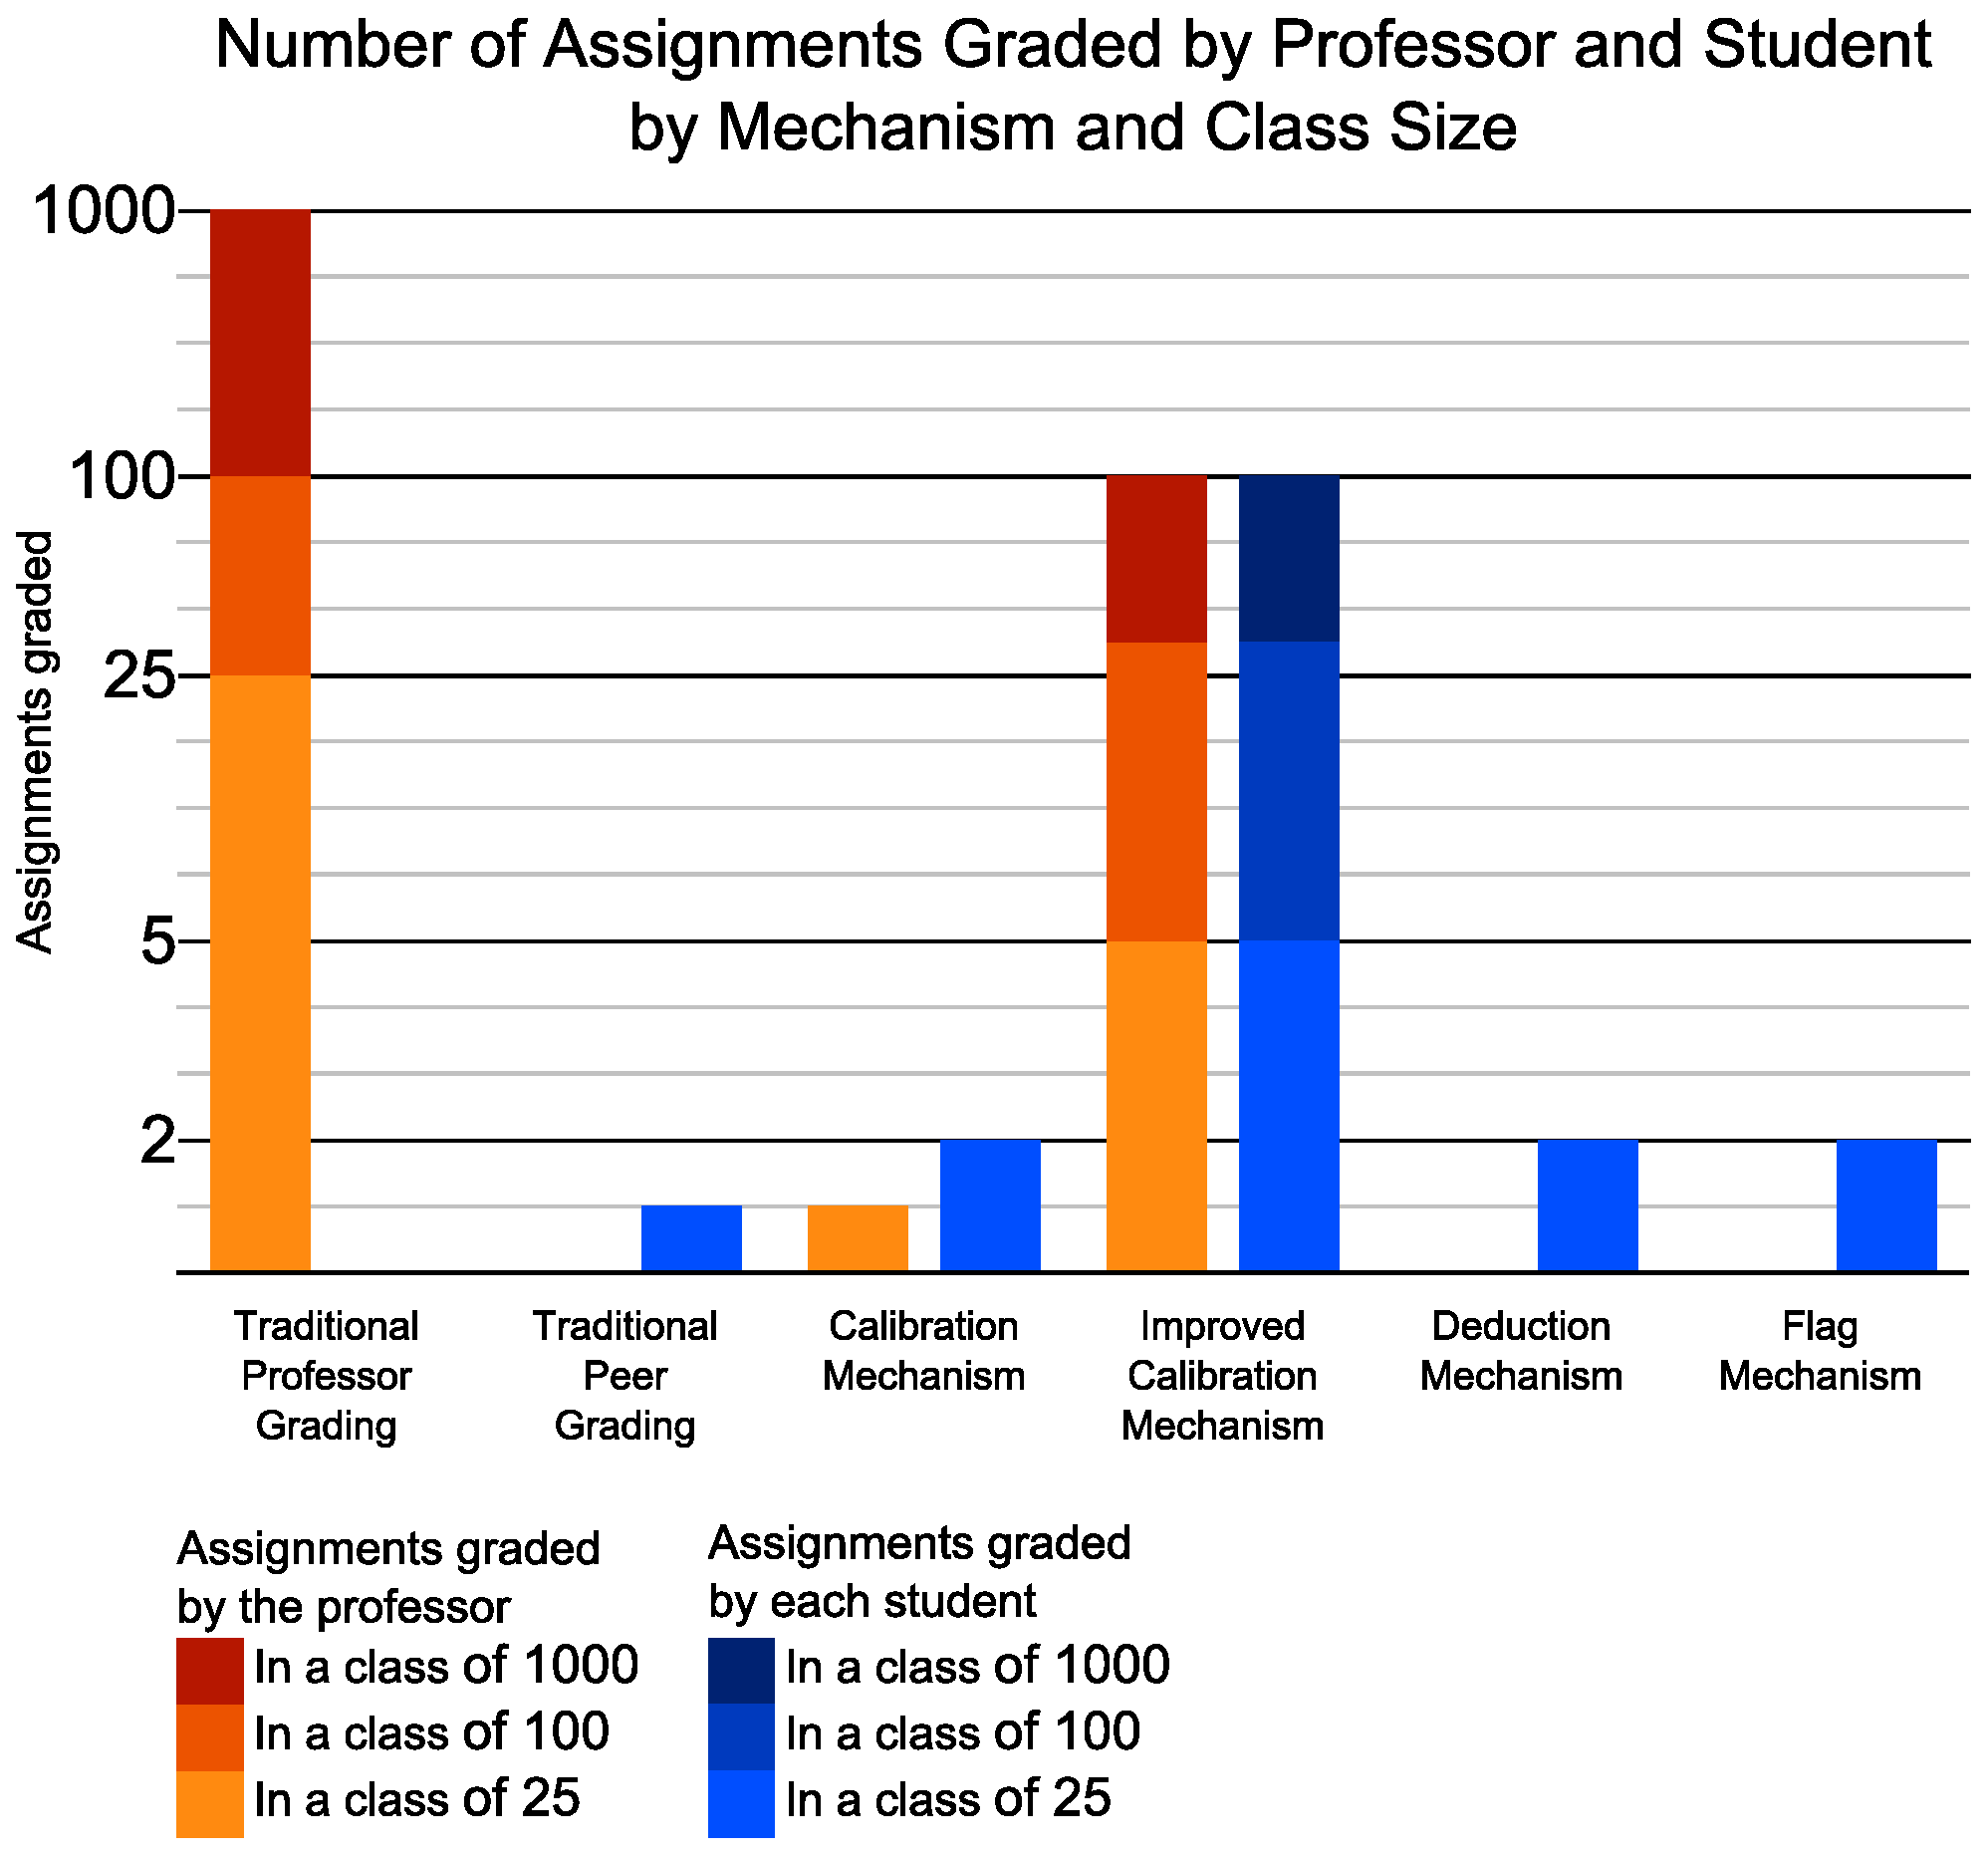
\includegraphics[width=\textwidth]{Chart.eps}
}
\begin{thebibliography}{9}

\bibitem{canmoocsreducecc}
  % http://sicet.org/journals/ijttl/issue1201/2_Ruth.pdf
  Ruth, S. (2012). \emph{Can MOOCs and existing e-learning paradigms help reduce college costs}? International Journal of Technology in Teaching and Learning, 8(1), 21-32.

\bibitem{makingsenseofmoocs}
  % http://www-jime.open.ac.uk/jime/article/viewArticle/2012-18/html
  Author,
  \emph{Title}.
  Source,
  Year.

\bibitem{swotanalysisofmoocs}
  % http://www.editlib.org/p/112020
  Author,
  \emph{Title}.
  Source,
  Year.

\bibitem{rightandwrongmoocs}
  % http://www.tonybates.ca/2012/08/05/whats-right-and-whats-wrong-about-coursera-style-moocs/
  Author,
  \emph{Title}.
  Source,
  Year.

\bibitem{boycottfinal}
  % http://www.insidehighered.com/news/2013/02/12/students-boycott-final-challenge-professors-grading-policy-and-get
  Author,
  \emph{Title}.
  Source,
  Year.

\bibitem{autograding}
  % http://www.ecu.edu/cs-acad/fsonline/customcf/committee/tg/2013proposals/08.pdf
  Author,
  \emph{Title}.
  Source,
  Year.

\bibitem{edxsoftware}
  % http://www.bostonmagazine.com/news/blog/2013/04/04/edx-now-has-robots-to-grade-your-essays/
  Author,
  \emph{Title}.
  Source,
  Year.

\bibitem{automatedsystemssuck}
  Herrington, A., \& Moran, C. (2012). \emph{Writing to a machine is not writing at all}. In N. Elliot \& L. Perelman (Eds.), Writing assessment in the 21st century: Essays in honor of Edward M. White (pp. 219-232). New York, NY: Hampton Press.

\bibitem{howaccurateispeergrading}
  % http://educationgroup.mit.edu/HHMIEducationGroup/wp-content/uploads/2011/05/Freeman-et-al-2010.pdf
  Author,
  \emph{Title}.
  Source,
  Year.
  
\bibitem{theproblemswithpeergradingincoursera}
%http://www.insidehighered.com/blogs/hack-higher-education/problems-peer-grading-coursera
Author,
  \emph{Title}.
  Source,
  Year.
  
\bibitem{robogradingproblems}
%http://bltnotjustasandwich.com/2013/04/05/the-problems-with-moocs-1-robo-essay-grading/
Author,
  \emph{Title}.
  Source,
  Year.
  
\end{thebibliography}
\end{document}
